\documentclass[10pt,letterpaper,final]{report}
\usepackage[margin=.75in]{geometry}
\usepackage[utf8]{inputenc}
\usepackage{amsmath}
\usepackage{amsfonts}
\usepackage{amssymb}
\usepackage{amsthm}
\renewcommand\qedsymbol{$\blacksquare$}
\usepackage{enumerate}
\usepackage{enumitem}
\usepackage{hyperref}
\usepackage{pdfpages}
\usepackage{graphics}
\usepackage{graphicx}
\usepackage{tikz}
\usepackage{tikz-qtree}
\usepackage{forest}
\usepackage{float}
\usetikzlibrary{automata,arrows}
\usetikzlibrary{shapes.multipart, positioning}
\usepackage{mdframed}
\usepackage[
  backend=biber,
  style=numeric-comp,
  sorting=none
]{biblatex}
\addbibresource{references.bib}

\usepackage{minted}
\usemintedstyle{algol_nu}
\usepackage{xltabular}
\usepackage{pdflscape}
\usepackage{tcolorbox}
\usepackage{enumitem}
\usepackage{array}
\usepackage{todonotes}
\setuptodonotes{inline}  % render \todo notes as full-width blocks in the text flow, not margin boxes

% Based on template from COSC-417 at Towson University, originally authored by Marius Zimand

% To input a script, adapt the following:
% \inputminted[breaklines, breakanywhere, fontsize=\footnotesize, frame=single, fontsize=\footnotesize]{python}{script.py}

\begin{document}
\begin{center}
  \fbox{
    \vbox{
      \begin{flushleft}
        Jonathan Llovet \\  % authors' names
        EN.625.252.81 \\  %class
        2026-08-31 \\  % date
        Module 1 - Homework 1 \\ % ID
      \end{flushleft}
      \center{\Large{\textbf{Linear Algebra}}}
      %\end{mdframed}
    } % end vbox
  } % end fbox
  \vline
\end{center}

\medskip

\noindent\textbf{Directions}

Complete the following problems showing all your work. You may use a calculator to check your work, but should write out (or \TeX up) all the steps of your solution. Please upload your work as a single .pdf file in the course.

\medskip
\noindent\textbf{Problem 1:}
\medskip

Find the general solution of the system below two ways:
\begin{enumerate}
  \item Row reduction by hand.
  \item Verify your answer using any program or calculator of your choice.
\end{enumerate}
Clearly state which program you used and include a screen shot of your code and output.

\medskip
\noindent\textbf{Answer:}
\medskip

\begin{align*}
  A & =
  \left[\begin{array}{rrr|r}
      1 & 3 & 4 & 7 \\
      3 & 9 & 7 & 6
    \end{array}\right]
    &      & \rho_2 \leftarrow \rho_2 + (-3)\rho_1
  \\[6pt]
    & \sim
  \left[\begin{array}{rrr|r}
      1 & 3 & 4  & 7   \\
      0 & 0 & -5 & -15
    \end{array}\right]
    &      & \rho_2 \leftarrow -\tfrac{1}{5}\rho_2
  \\[6pt]
    & \sim
  \left[\begin{array}{rrr|r}
      1 & 3 & 4 & 7 \\
      0 & 0 & 1 & 3
    \end{array}\right]
    &      & \rho_1 \leftarrow \rho_1 + (-4)\rho_2
  \\[6pt]
    & \sim
  \left[\begin{array}{rrr|r}
      1 & 3 & 0 & -5 \\
      0 & 0 & 1 & 3
    \end{array}\right]
\end{align*}

The equivalent system to the final augmented matrix is:

\begin{alignat*}{4}
  x_1 & {}+{} & 3x_2 &       &     & {}={} & -5 \\
      &       &      & \quad & x_3 & {}={} & 3
\end{alignat*}

Solving the first equation for $x_1$:

\begin{align*}
  x_1 & = -5 - 3x_2
\end{align*}

Hence, a parameterized description of the system $A$ is:
\[
  \begin{cases}
    x_1 & = -5 - 3x_2    \\
    x_2 & \text{is free} \\
    x_3 & = 3
  \end{cases}
\]

The procedure for row reduction can be found in \parencite{LayEtAl2020LinearAlgebraAndItsApplications}, \parencite{jhuwse625-252-module-01-lectures}.

\pagebreak

I used the following tools to validate my solution programmatically. I tried out a few options to see what is available among deterministic tools, since some are useful for pedagogic purposes and some are useful for performing calculations.

Here I am using a tool at \url{https://matrixcalc.org} that solves and explains the derivation of the general solution, with the option of selecting specific algorithms. This site has a number of useful tools for matrix operations.

\begin{figure}[H]
  \centering
  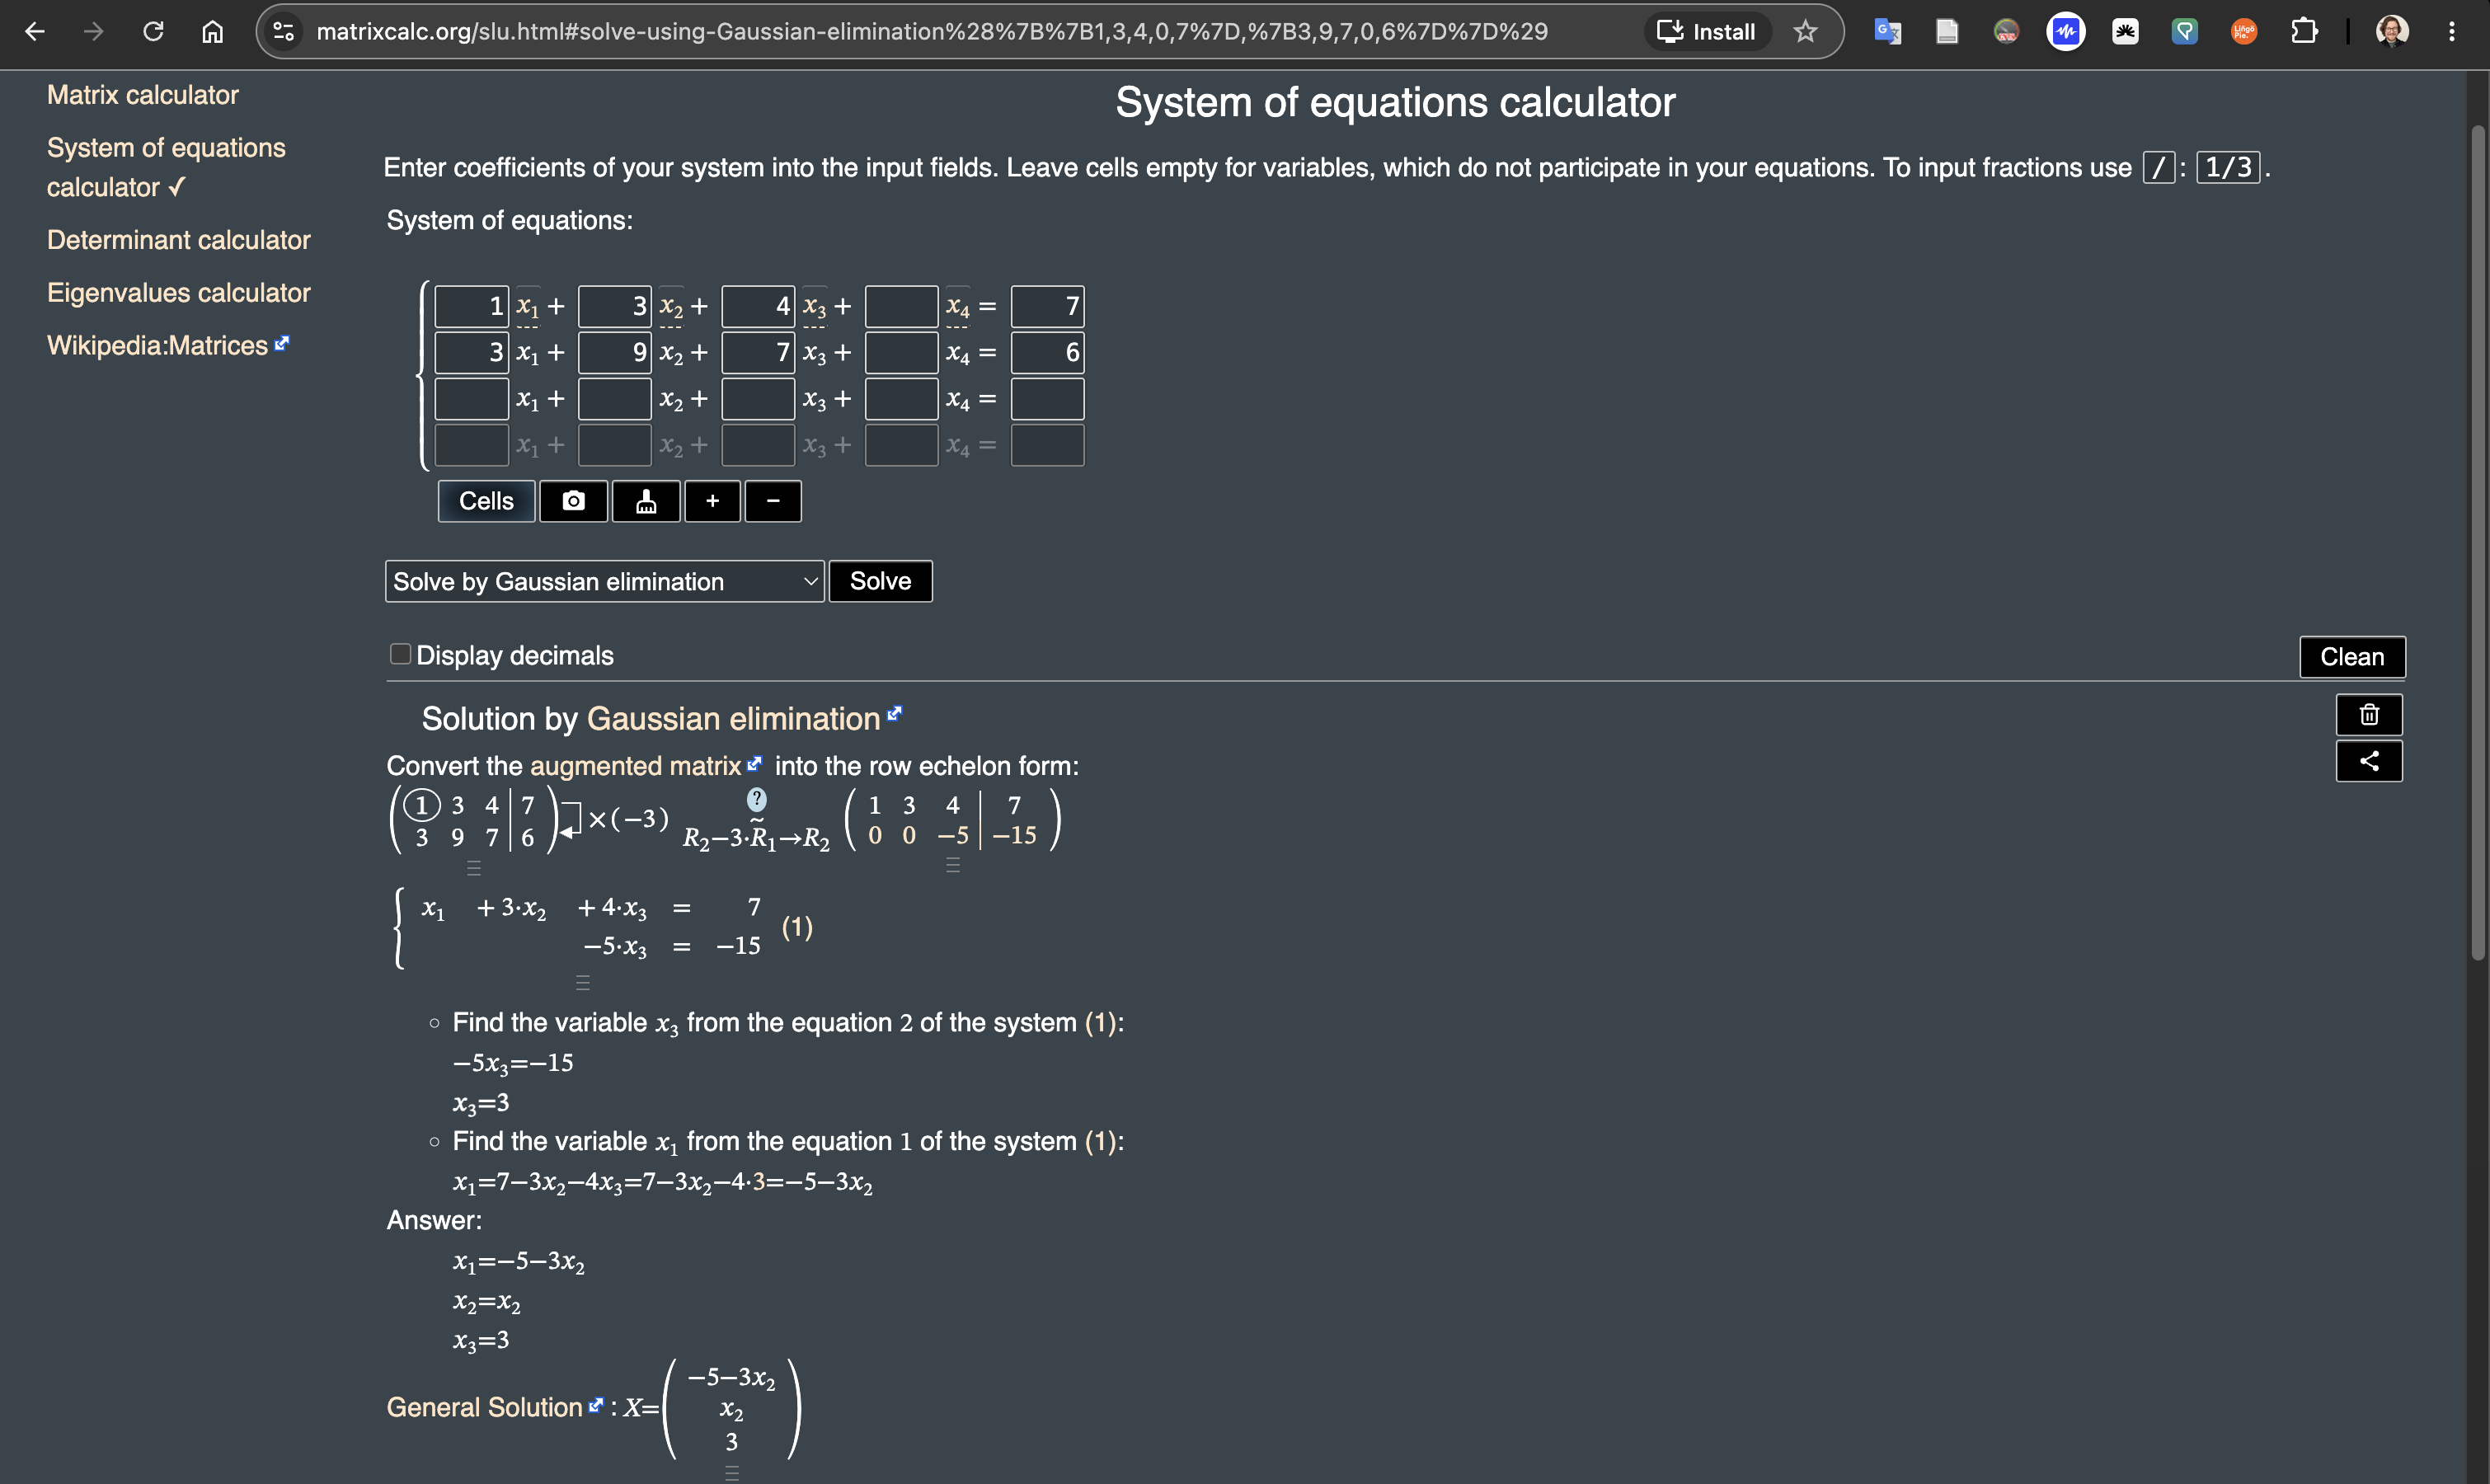
\includegraphics[width=\textwidth,page=1]{2026-09-04-systems-of-equations-calculator.png}
  \caption{System of Linear Equations Calculator \cite{MatrixcalcSystemOfLinearEquations}}\label{fig:matrix-system-of-linear-equations-calculator}
\end{figure}

\pagebreak
Here is a partial solution produced by a TI-84 emulator at \url{https://ti84calculator.io/}, reducing the matrix to reduce row echelon form through the built in \texttt{rref} function. While this has the advantage that it can also be done offline using a physical calculator or one of a large number of emulators, it does leave some additional work to be done, since the reduced row echelon form still must be converted into an expression of a parametric solution to the system. The repository for the emulator can be found in \cite{GitHubGitHubBifduTICalculator}.

\begin{figure}[H]
  \centering
  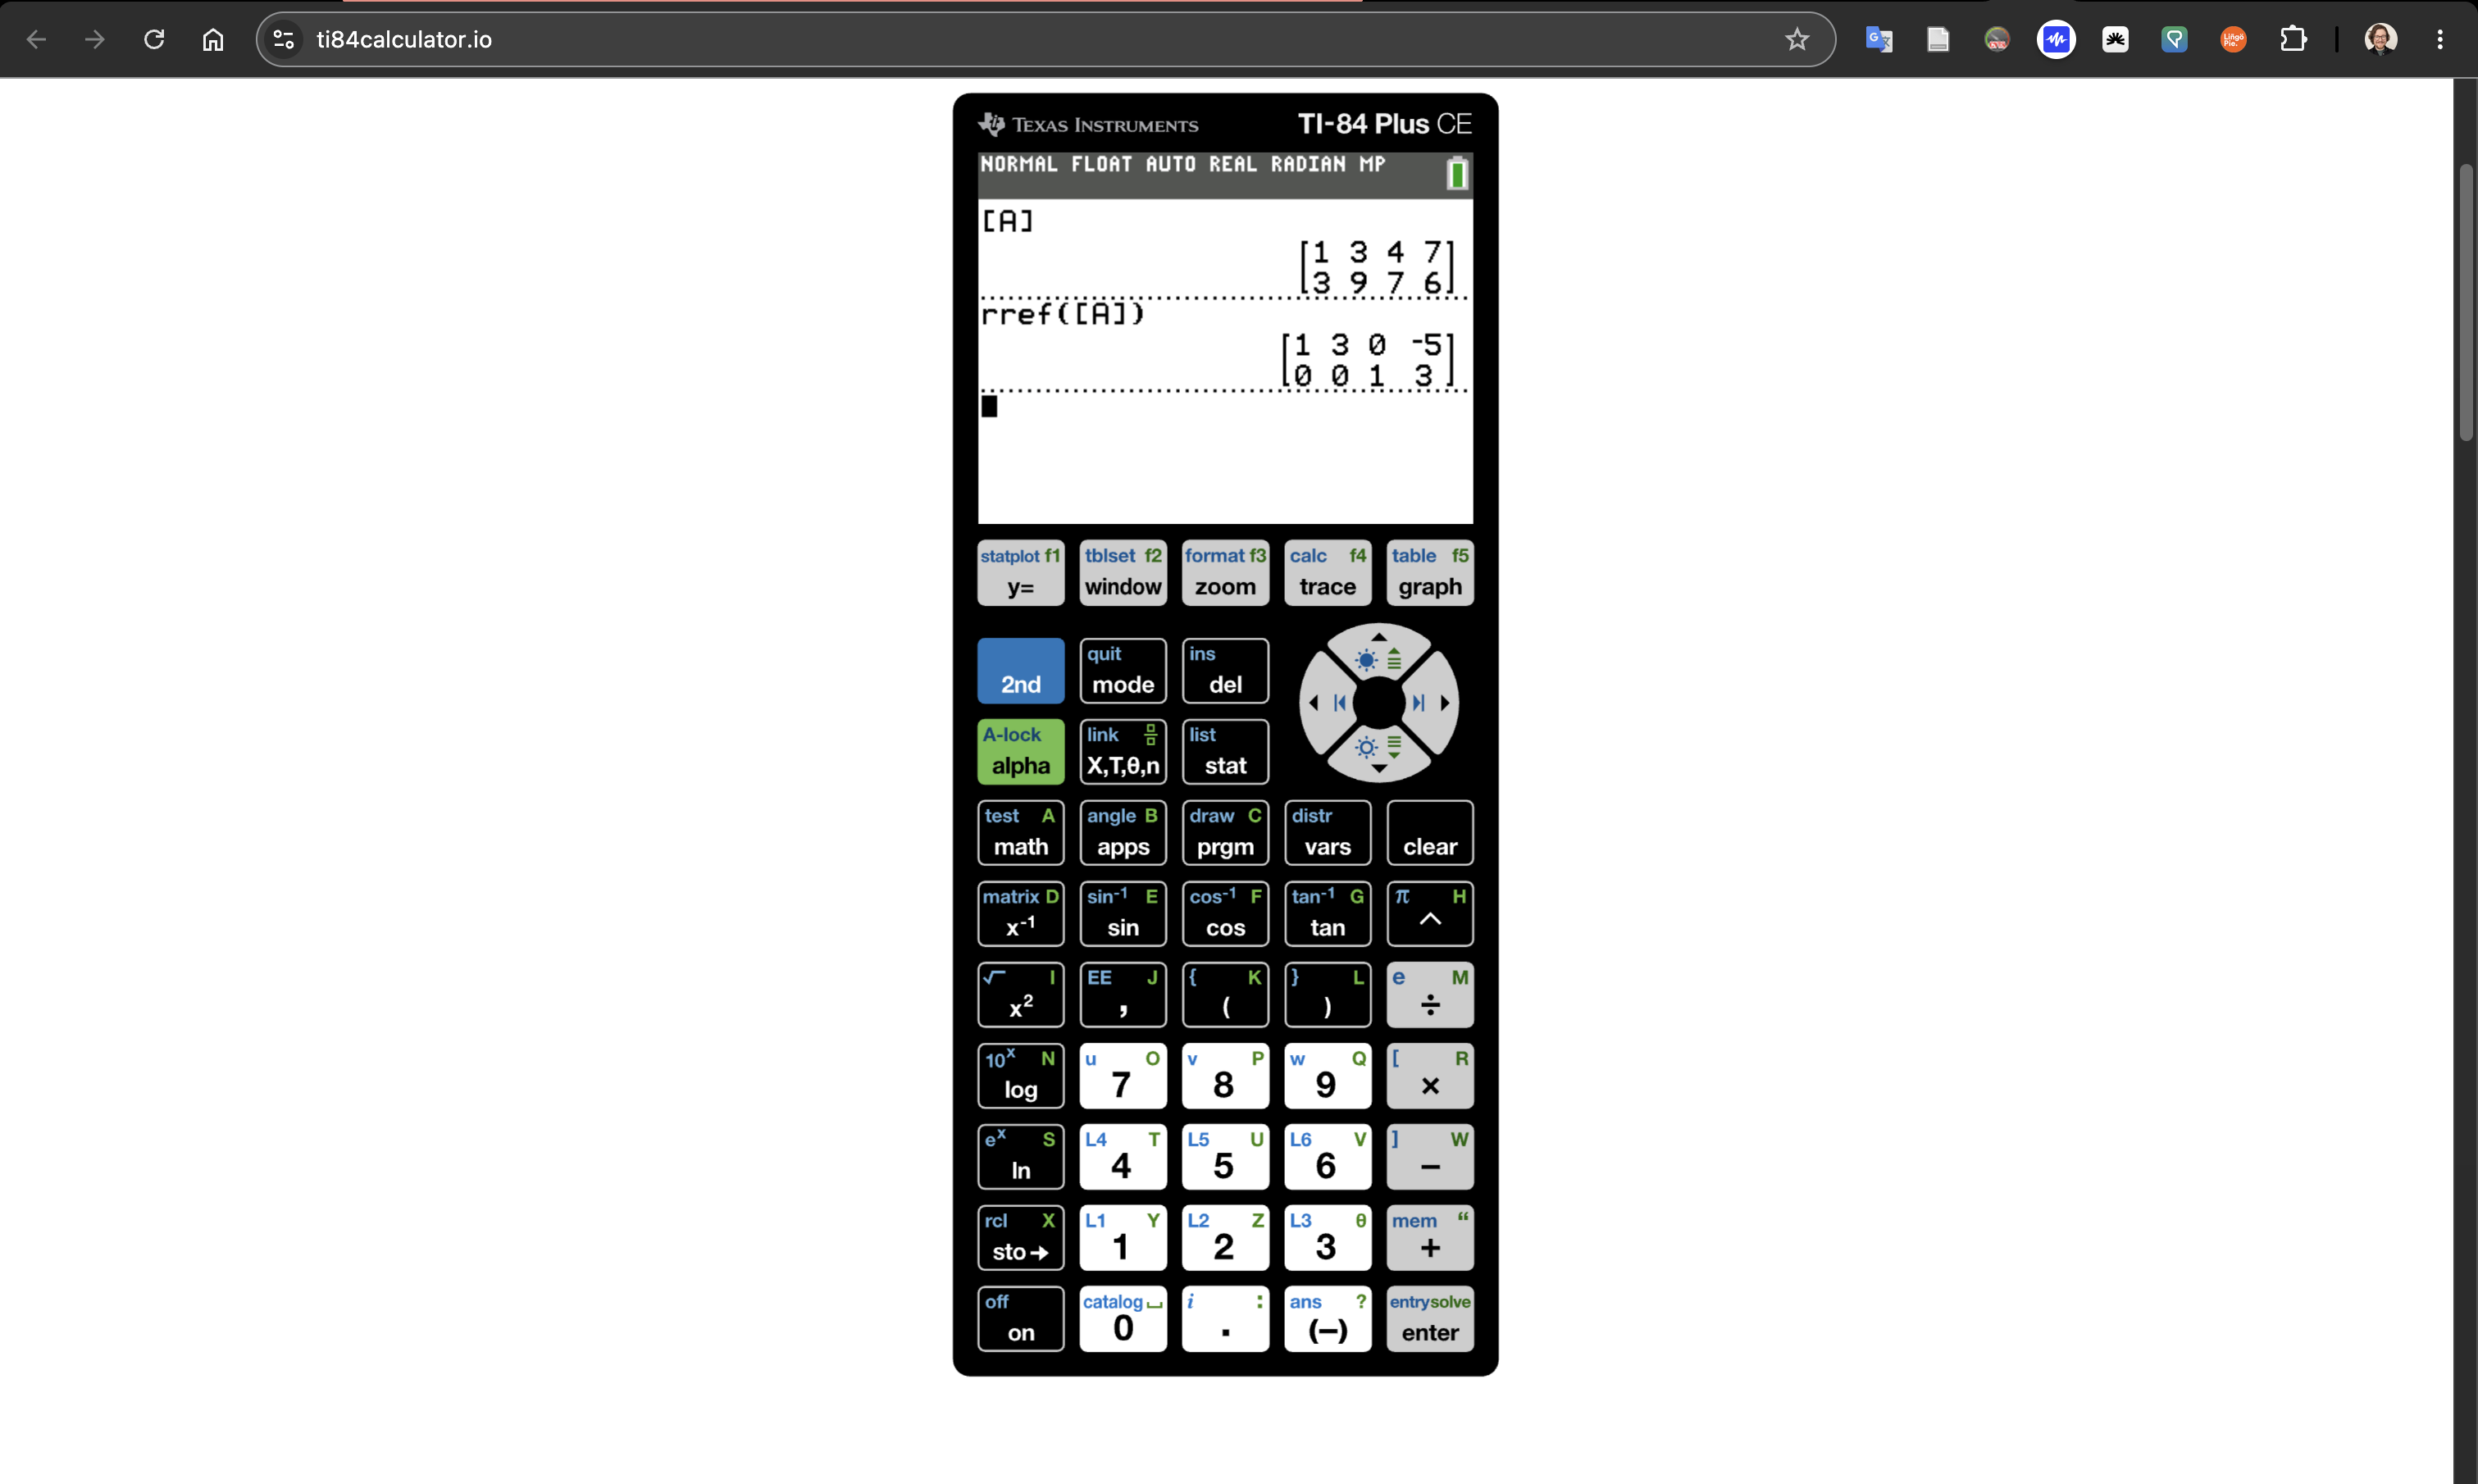
\includegraphics[width=\textwidth,page=1]{2026-09-04-ti-84-emulator.png}
  \caption{TI-84 Emulator \cite{TI84CalculatorIO}}\label{fig:ti84-calculator-online-emulator}
\end{figure}

In addition to these, I re-explored using SymPy, a package for symbolic mathematics in Python. I asked Claude \cite{Anthropic2026ClaudeOpus48} to provide me a brief demo, and then I read SymPy documentation at \cite{DocssympyorgMatricesSymPy} \cite{Sympy10.7717/peerj-cs.103} to write a short script to solve the system. I plan to spend more time with SymPy and similar libraries across languages in the future, both for applications such as building automated reasoning tools and for doing research and work in various areas of mathematics.

\inputminted[breaklines, breakanywhere, fontsize=\footnotesize, frame=single, fontsize=\footnotesize]{python}{solve.py}

\pagebreak
\noindent\textbf{Problem 2:}
\medskip

What would you have to know about the pivot columns in an augmented matrix in order to know that the linear system is consistent and has a unique solution? Explain in complete sentences and provide examples to justify your reasoning.

\medskip
\noindent\textbf{Answer:}
\medskip

Recall Theorem 2 from \citetitle{LayEtAl2020LinearAlgebraAndItsApplications}, which says:

\begin{tcolorbox}[colback=blue!10!white, colframe=blue!80!black, title=Theorem 2 - Existence and Uniqueness Theorem]
  A linear system is consistent if and only if the rightmost column of the augmented matrix is \emph{not} a pivot column - that is, if and only if an echelon form of the augmented matrix has \emph{no} row of the form
  \begin{align*}
    [\ 0 \ldots 0\ \ b\ ] \text{ with $b$ nonzero}
  \end{align*}
  If a linear system is consistent, then the solution set contains either (i) a unique solution, when there are no free variables, or (ii) infinitely many solutions, when there is at least one free variable.
\end{tcolorbox}

\medskip

By this theorem, when the linear system is consistent and it has a unique solution, there are no free variables. What do we have to know about the pivot columns for this to be the case? In order to answer this it will be easier to think about the structure of the matrix rows as well. A free variable can be identified when a matrix is in reduced row echelon form (RREF). Within a given row of a matrix in RREF, if there are any coefficients to the right of that row's pivot variable (if there is a pivot variable in the row), then those coefficients are free variables.

Consider the matrix $A$ below. Let the black squares $\blacksquare$ indicate that a position $A_{i,j}$ is a pivot position in row $i$, column $j$. In RREF, this means that each element in a $\blacksquare$ position is equal to $1$. Let the value $\star$ indicate that that there is a value $x$ at $A_{i,j}$, such that $x \in D$, where $D$ is the domain of the elements of $A$.

\begin{align*}
  A & =
  \left[\begin{array}{rrr|r}
      \blacksquare & 0            & 0            & \star \\
      0            & \blacksquare & 0            & \star \\
      0            & 0            & \blacksquare & \star
    \end{array}\right]
\end{align*}

Presume there is a matrix $A_0$ in RREF, and that we have replaced the elements at the positions with $\blacksquare$ with $1$. Let each of the stars be replaced by a variable $a,b,c \in D$, where $D$ is the domain of the elements of $A$. Performing these replacements:

\begin{align*}
  A_0 & =
  \left[\begin{array}{rrr|r}
      1 & 0 & 0 & a \\
      0 & 1 & 0 & b \\
      0 & 0 & 1 & c
    \end{array}\right]
\end{align*}

Having a matrix in the form of $A_0$ is the best-case scenario for us in determining that there is a unique solution to the system of equations, because a matrix in RREF is unique among the class of matrices that are equivalent under the set of elementary row operations. In this form, the solution to the system of equations can be read off from the matrix, in a way similar to how the values of a boolean function can be read off from a truth table in conjunctive normal form. In RREF, the following characteristics hold:

\begin{enumerate}
  \item The final column is not a pivot column (by Theorem 2)
  \item Each pivot column has a single nonzero value $1$
  \item The pivot column is the location of the leftmost nonzero value in the row
  \item In each pivot column, if there are rows above or below the pivot position, the values of elements in those positions will be $0$
\end{enumerate}

If these characteristics were not to hold, then a) the system would not be in RREF, or b) it would have infinitely many solutions, or c) it would have no solution. In the first case, the matrix would be reducible to RREF through a set of elementary row operations, since there are other matrices that are equivalent to $A$, namely $\{X \in M_A, \mid X \sim A\}$, where $M_A$ is the class of matrices that can be obtained through the elementary row operations of scaling, swapping, and row addition.

Consider the matrix $B$ below.

\begin{align*}
  B & =
  \left[\begin{array}{rrr|r}
      \blacksquare & \star        & \star        & \star \\
      \star        & \blacksquare & \star        & \star \\
      \star        & \star        & \blacksquare & \star
    \end{array}\right]
\end{align*}

If $B \in M_A$, then $B = F(A)$, where $F$ is a some composition of elementary row operations. Because of the closure of the class of matrices $M_A$ under the elementary row operations, there are infinitely many unique matrices that are equivalent to $A$ and for which the matrix $A$ is a characteristic, fully simplified matrix.

What are ways that they look? Let each of the black squares in $A$ be replaced by the value $1$. Further, let each of the stars be replaced by a variable $a,b,c \in D$, where $D$ is the domain of the elements of $A$. The composition of elementary row operations transforms $A_0$ into other equivalent matrices. An example is shown below. The inverse process is what row reduction into RREF performs, though this does not have to be in exactly the reverse sequence composition $F$ of row operations transformations from $A_0$ to another matrix $B$.

\begin{align*}
  A_0 & =
  \left[\begin{array}{rrr|r}
      1 & 0 & 0 & a \\
      0 & 1 & 0 & b \\
      0 & 0 & 1 & c
    \end{array}\right]
  \\[6pt]
      & \sim
  \left[\begin{array}{rrr|r}
      1 & 2 & 0 & a + 2b \\
      0 & 1 & 0 & b      \\
      0 & 0 & 1 & c
    \end{array}\right]
      & \rho_1 \leftarrow \rho_1 + (2)\rho_2
  \\[6pt]
      & \sim
  \left[\begin{array}{rrr|r}
      1 & 2 & 0 & a + 2b \\
      0 & 1 & 3 & b + 3c \\
      0 & 0 & 1 & c
    \end{array}\right]
      & \rho_2 \leftarrow \rho_2 + (3)\rho_3
  \\[6pt]
      & \sim
  \left[\begin{array}{rrr|r}
      1 & 2 & 0 & a + 2b      \\
      0 & 1 & 3 & b + 3c      \\
      2 & 4 & 1 & 2a + 4b + c
    \end{array}\right]
      & \rho_3 \leftarrow \rho_3 + (2)\rho_1
\end{align*}

Consider next the situation where for some matrix $C$, where $C \not\in M_A$. This means that there is no sequence $F: C \to A$ of elementary row operations that could transform $C$ to $A$ while maintaining the equivalence of the systems represented. If this were the case and also there were no row in $C$ of the form $[\ 0 \ldots 0\ \ b\ ] \text{ with $b$ nonzero}$, then $C$ would have infinitely many solutions, again by Theorem 2. In such a case, there would be free variables in $C$, where there would be non-zero coefficients to the right of pivot positions that could not be reduced to zero by the elementary row operations. Take for example matrix $C$ below, where the variables $a,b \ne 0$:

\begin{align*}
  C & =
  \left[\begin{array}{rrrrr|r}
      \blacksquare & a     & \star        & \star & \star        & \star \\
      \star        & \star & \blacksquare & b     & \star        & \star \\
      \star        & \star & \star        & \star & \blacksquare & \star
    \end{array}\right]
\end{align*}

The matrix $C$ above could be reduced to echelon form, but not to reduced row echelon form. There is no single characteristic matrix for this system, because there is not a unique solution. Finally, in the final case, wherethere is another matrix $X \not\in M_A$, where $X$ has a pivot column where the row containing the pivot position is of the form $[\ 0 \ldots 0\ \ b\ ] \text{ with $b$ nonzero}$, the system $X$ is inconsistent, by Theorem 2. See the example inconsistent system $X$ below.

\begin{align*}
  X & =
  \left[\begin{array}{rrr|r}
      \star & \star & \star & \star \\
      \star & \star & \star & \star \\
      0     & 0     & 0     & 1
    \end{array}\right]
\end{align*}

\pagebreak

\noindent\textbf{Problem 3:}
\medskip

Consider the linear system:

\begin{align*}
  x_1  + hx_2 & = 2 \\
  4x_1 + 8x_2 & = k
\end{align*}

\begin{enumerate}
  \item Find values of $h$ and $k$ such that the system has no solution.
  \item Find values of $h$ and $k$ such that the system has a unique solution.
  \item Find values of $h$ and $k$ such that the system has infinitely many solutions.
\end{enumerate}


\medskip
\noindent\textbf{Answer:}
\medskip

Let the given system be referred to as $A$, and let it be represented as the following matrix:

\begin{align*}
  A & =
  \left[\begin{array}{rr|r}
      1 & h & 2 \\
      4 & 8 & k
    \end{array}\right]
\end{align*}

\begin{enumerate}
  \item No Solution

        To find a system with no solution, we can lean on Theorem 2, which tells us that we have a system with no solution if there is a row such that the pivot $b$ is in the final position (i.e. the last element in the row), $b \ne 0$, and all the preceding elements in the row are equal to $0$. Let us transform the given system $A$ as follows:
        \begin{align*}
          A & =
          \left[\begin{array}{rr|r}
              1 & h & 2 \\
              4 & 8 & k
            \end{array}\right]
          \\[6pt]
            & \sim
          \left[\begin{array}{rr|r}
              1 & h    & 2   \\
              0 & 8-4h & k-8
            \end{array}\right]
            & \rho_2 \leftarrow \rho_2 + (-4)\rho_1
        \end{align*}
        Now, concretely, we can ask: under what conditions is the equation $8 - 4h = k - 8$ inconsistent? If one side of the equation equals $0$ while the other does not, then we have found what we are looking for. If $h = 2$, then $8 - 4h = 0$. Then the system is inconsistent $\forall k \in \mathbb{R} \mid k \ne 8$. Take for example $h=2, k=9$. Then the system $A$ is:
        \begin{align*}
          A & =
          \left[\begin{array}{rr|r}
              1 & h      & 2   \\
              0 & 8-4(2) & 9-8
            \end{array}\right]
          \\[6pt]
            & \sim
          \left[\begin{array}{rr|r}
              1 & 2 & 2 \\
              0 & 0 & 1
            \end{array}\right]
        \end{align*}
        This is inconsistent by Theorem 2, QED.

  \item Unique Solution

        Here we can reuse work from the last question. Consider again this transformation of the sytem $A$:

        \begin{align*}
          A & =
          \left[\begin{array}{rr|r}
              1 & h & 2 \\
              4 & 8 & k
            \end{array}\right]
          \\[6pt]
            & \sim
          \left[\begin{array}{rr|r}
              1 & h    & 2   \\
              0 & 8-4h & k-8
            \end{array}\right]
            & \rho_2 \leftarrow \rho_2 + (-4)\rho_1
        \end{align*}
        To satisfy Theorem 2, we must have the matrix in echelon form, so that $8-4h \ne 0$, so that the rightmost value is not a pivot. If we have the system in echelon form, then we must consider a value for $h$ that satisfies the constraint that there are no free variables. In order for that to be the case in row 1, $h$ must equal $0$. Let the final matrix above be $A_0$. Substituting in $h=0$ into $A_0$:

        \begin{align*}
          A_0 & =
          \left[\begin{array}{rr|r}
              1 & 0 & 2   \\
              0 & 8 & k-8
            \end{array}\right]
          \\[6pt]
              & \sim
          \left[\begin{array}{rr|r}
              1 & 0 & 2             \\
              0 & 1 & \frac{k-8}{8}
            \end{array}\right]
              & \rho_2 \leftarrow \tfrac{1}{8}\rho_2
        \end{align*}

        The equation corresponding to the final row is satisfied $\forall k \in \mathbb{R} \mid k \ne 8$. This gives us the answer to our next question. Here, though, how can we constrain the system to a single solution? If $k = 8$, then $\tfrac{k-8}{8} = \frac{0}{8} = 0$. This means that the only solution to the system when $h=0, k=8$ is $(2, 0)$, QED.

  \item Infinitely Many Solutions

        Consider the original given system again:

        \begin{align*}
          A & =
          \left[\begin{array}{rr|r}
              1 & h & 2 \\
              4 & 8 & k
            \end{array}\right]
        \end{align*}
        Here we want to contrive to have a free variable, since per Theorem 2, there are infinitely many solutions if the system is consistent and has at least one free variable. A free variable is a variable that is not equal to $0$ when the system is in RREF. Since $k$ is in the final position, we must try to eliminate it, along with the other values from the second row. To do so, first let $h = 2$. Then we can perform a row reduction on the system.

        \begin{align*}
          A & =
          \left[\begin{array}{rr|r}
              1 & 2 & 2 \\
              4 & 8 & k
            \end{array}\right]
          \\[6pt]
            & \sim
          \left[\begin{array}{rr|r}
              1 & 2 & 2   \\
              0 & 0 & k-8
            \end{array}\right]
            & \rho_2 \leftarrow \rho_2 + (-4)\rho_1
        \end{align*}

        We are most of the way there. To preserve the consistency of this system, we must avoid having row two have a pivot in the final position. Consequently, we must contrive that $k-8 = 0$, which is satisfied when $k=8$. The system then reduces to

        \begin{align*}
          A_1 & =
          \left[\begin{array}{rr|r}
              1 & 2 & 2 \\
              0 & 0 & 0
            \end{array}\right]
        \end{align*}

        In this system, there is a free variable, namely $x_2$, which means that there are infinitely many solutions, QED.
\end{enumerate}

\pagebreak


\section*{Source Code}
The full source code, including LaTeX, tooling, other artifacts, and git history is available on my Github repository for the class here:
\begin{center}
  \url{https://github.com/jllovet/jhu-en-625-252-fa26-linear-algebra}
\end{center}

\printbibliography

\end{document}
